\chapter{Strategies Evaluation}
\label{chap:strategies}

\section{Modelisation}
\subsection{Metrics}
A way to rationaly compare strategies is needed in order to discuss their
relative strengths and weaknesses. Three main characteristics will be used for
that:
\begin{itemize}
        \item latency;
        \item number of nodes;
        \item overhead.
\end{itemize}

\subsubsection{Latency}
The latency is the number of messages needed to finalize a block. Ideally, you
want to have a latency as low as possible to reach finality as soon as possible.
The latency is a way to measure liveness in a blockchain system. If it is low,
then the system is considered more "live", as less messages are needed in order
to confirm a transaction, and therefore less time.
\todo{schema for latency}

\subsubsection{Number of nodes}
The number of nodes is quite straightforward; it is the number of nodes that can
be included in the validator set. This number should be as high as possible to
guarantee decentralization and therefore safety.
\todo{schema for number of nodes}

\subsubsection{Overhead}
The overhead is the number of messages that are sent over the network between
one step of the consensus and the next. It should be as low as possible to keep
the costs in bandwidth low.
\todo{schema for overhead}


\subsection{Tradeoff triangle/Trilemma}
In a standard consensus protocol, the three metrics form a trade-off triangle in
kind of a "pick two" fashion. \todo{not a pick two} \gls{cbc}-Casper has no assumptions on timings,
sources, contents, destinations of the messages that are exchanged, and can
therefore explore the whole trade-off space. This project aims to find
strategies that span the entierty of the triangle and 

\subsection{Model}
The model that has been chosen for the evaluation is the following:
\[1 = s_n \cdot \frac{1}{n} + s_l\cdot l + s_o\cdot o\]
This model binds 3 scores \(s_x\) to their respective variables \(x\).
Variables are as follows:
\begin{itemize}
    \item \(n\) the number of nodees;
    \item \(l\) the latency;
    \item \(o\) the overhead.
\end{itemize}
The higher the score \(s_x\) is, the more its related variable is preponderant
in the strategy and therefore the closer to a corner of the triangle the strategy is.
\todo{why 1/n, why everything linear?}

\subsection{Model Evaluation}
After running the strategies in the simulation environment, metrics for \(n\),
\(l\) and \(o\) will be recorded. Then, for multiple runs, a linear regression
will be performed in order to find the scores \(s_x\).

\section{Strategies}
\label{sec:strategies}

The following strategies were proposed in order to visit the entierty of the
trade-off triangle:
\begin{itemize}
        \item round-robin;
        \item randomness;
        \item double round-robin;
        \item overhead.
\end{itemize}
These strategies should allow one to visit the whole triangle and to discuss
their respective strength and weaknesses. The following sections describe the
strategies as well as their expected locations in the triangle.

\subsection{Round-robin}
The first strategy that comes to mind is a simple round-robin. Nodes send
messages one after the other, in a fixed order.
\todo{talk about real life implications? aka synchronize all nodes?,\ldots and
that for every strategy}

\subsection{Randomness}
The next strategy is the simplest to think of: complete randomness. Using fixed
probability density functions, nodes chose when to create messages and to which
other validator to send them.

\subsection{Double Round-robin}
In this setting, two nodes send messages at the same time, in a fixed order. If
the two nodes that send messages at the same step are at opposite places in the
set of validators \todo{explain better}, the latency to finality is supposedly
half as much as the simple round-robin strategy. The overhead is however
doubled.\todo{add that we could have a triple rr, quadrr, \ldots}

\subsection{Maximal Overhead}
This strategy is the most expensive in terms of bandwidth; at each step, each
validator sends a message to the others. This example strategy should give a
baseline value for the maximum overhead that is reachable in the tradeoff
triangle.

\subsection{Bottom-up strategies}
\todo{talk about strategies that are obtained from a bottom-up point of view,
instead of a global vision, each node decides when and why it has to send a
message}
\todo{talk about incentives, slashing and such}

\section{Experimentations}
Over the duration of this thesis, the \texttt{core-cbc} library has included a
test framework called \texttt{proptest}. The testing framework that has been
implemented includes ways to simulate the behavior of the Casper protocol over
multiple nodes and thousands \todo{numbers} of blocks. At the time of the
writing, the simulations do not include networking latencies.

\subsection{\texttt{proptest}}
The \texttt{proptest} implementation is able to run blockchain simulations off
the following parameters:
\begin{itemize}
    \item Number of validators;
    \item Ending condition;
    \item Sender strategy;
    \item Receiver strategy.
\end{itemize}

\subsubsection{Number of validators}
This parameter is quite straightforward, it is the number of nodes that can
validate blocks.

\subsubsection{Ending condition}
The ending condition is a predicate that tells whether or not the simulation has
reached an end. In our case, the end of the simulation is reached when at least
one node finds a safety oracle for a blockchain that has an height of 4.
\todo{why 4}

\subsubsection{Sender strategy}
The sender strategy selects one or more nodes that will create new messages and
forward them to the rest of the network. All the basic strategies that have been
presented in Section~\ref{sec:strategies} are implemented as Sender strategies.
New strategies (including bottom-up ones) can be easily implemented as well.

\subsubsection{Receiver strategy}
Receiver strategies select a set of validators that receive messages created by
Sender strategies. Two strategies have been implemented for now: 
\begin{itemize}
        \item All receivers;
        \item Some receivers.
\end{itemize}

The \textit{all receivers} strategy broadcasts messages to each other validator.
The \textit{some receivers} strategy sends a message to \(1\) or more validator,
using an uniform probability density function.  As of now, none of the
implemented strategies are a good modelisation of a typical Ethereum network and
this will be fixed at a later iteration.  Nonetheless, these strategies offer
two extreme points on the spectrum of the network topology: a fully connected
one without latency (\textit{all receivers}), and a random one (\textit{some
receivers}) and will be both taken into account to compare the sender
strategies.

\todo{schema with what to measure}
\todo{how the measurements take place in the code}

\section{Visualization}
\begin{figure}
	\centering
	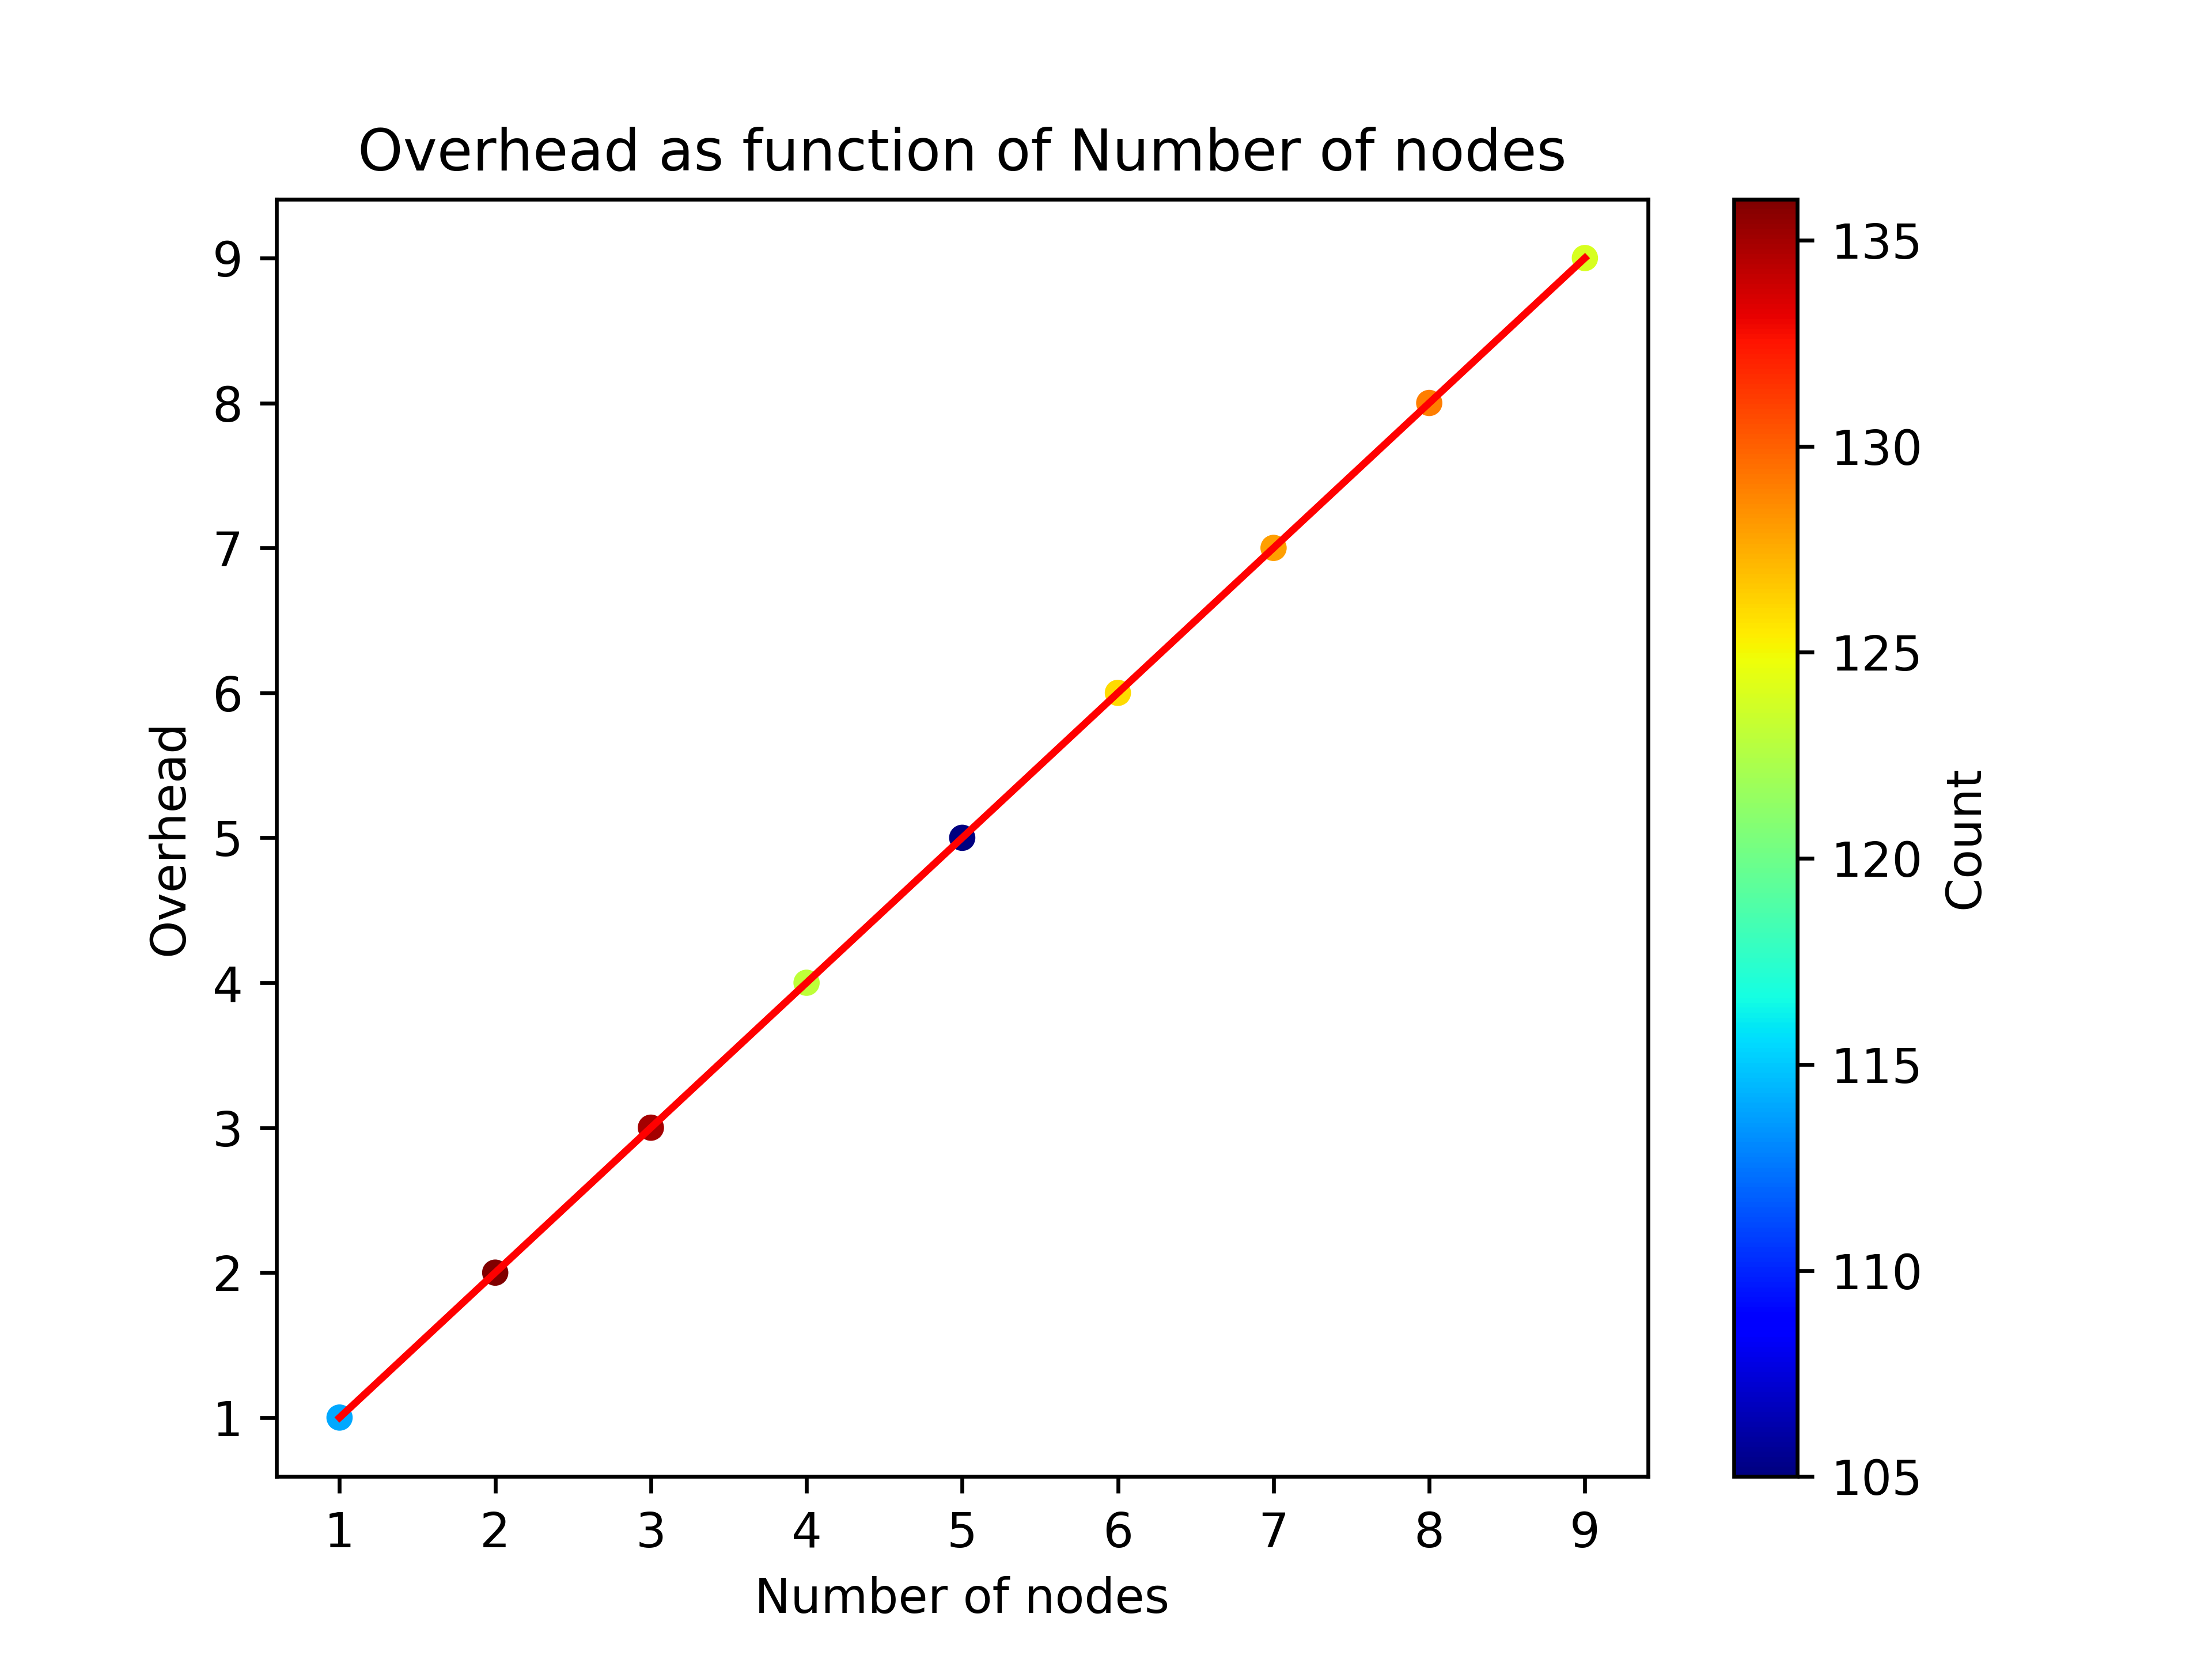
\includegraphics[width=0.8\columnwidth]{truc}
  \captionsetup{justification=centering}
  \caption{exmaple}
	\label{fig:asdasdasdasd}
\end{figure}

